% =====================================================================
%  Technical Report: LLM-Assisted Mobile Robot Task Planning
%  IEEEtran conference template, two-column, <= 4 pages (excl. refs)
% =====================================================================
\documentclass[conference]{IEEEtran}

\usepackage{cite}
\usepackage{amsmath,amssymb,amsfonts}
\usepackage{graphicx}
\usepackage{textcomp}
\usepackage{booktabs}
\usepackage{tikz}
\usetikzlibrary{arrows.meta,positioning}
\usepackage[hidelinks]{hyperref}

% ---------- Title / Author ----------
\title{LLM-Assisted Mobile Robot Task Planning in Simulation:\\
       From Natural Language to Validated Skill Sequences}

\author{\IEEEauthorblockN{Ruijie Zhu}
\IEEEauthorblockA{Department of Electromechanical Engineering\\
University of Macau, Macau, China\\
Email: mc65809@um.edu.mo}
}

\begin{document}

\maketitle

% ---------- Abstract ----------
\begin{abstract}
We present a simulated mobile robot system that converts natural-language
instructions into validated sequences of robot skills. A task planner, either
rule-based or driven by a large language model (LLM) with OpenAI-compatible
function calling, proposes calls to a fixed allowlist of navigation skills.
A validator and executor enforce argument types, workspace bounds, mutual
exclusion, and timeouts before the robot moves, and each skill returns a
structured result with measurable error metrics that drive bounded recovery
(retry once, reject, or stop and report). Experiments in Webots with a
TurtleBot3 show all required requests succeed with position and heading
errors within $0.1$\,m and $0.1$\,rad, invalid locations are rejected without
moving the robot, and malformed LLM arguments are intercepted by the
validator.
\end{abstract}

% =====================================================================
% I. INTRODUCTION
% =====================================================================
\section{Introduction}
This work tackles the problem of turning natural-language instructions into
safe, executable robot tasks. The system takes a request such as
``\emph{Go to storage, then visit the workbench, and stop.}'',
and produces a small plan, validated before execution, that the robot
carries out safely in a Webots simulation.

Existing LLM-based robot systems have shown that language can guide
action planning, but directly mapping unconstrained model outputs to robot
execution is risky: an LLM may emit syntactically valid yet physically
infeasible commands, invalid parameters, or sequences that do not terminate
as expected. This creates a gap between the flexibility of high-level
language reasoning and the reliability required by low-level robot
execution. This work therefore separates high-level task planning from
deterministic robot execution through a constrained skill interface and a
validation layer: the model suggests, but deterministic rules decide what is
executed.

The design is guided by four goals:
\begin{itemize}
  \item \textbf{Safety:} the LLM may only \emph{suggest} skill calls through
        a fixed allowlist of three skills. Every call is validated before it
        reaches the robot, and the LLM can never issue velocity commands or
        execute arbitrary code.
  \item \textbf{Explicit contracts:} each skill defines typed parameters with
        valid ranges, preconditions, a success condition with a timeout, and
        a structured result containing at least \texttt{success}, \texttt{reason},
        and elapsed time.
  \item \textbf{Reliable navigation:} target reaching is reported only when the
        robot is within a stated position \emph{and} heading tolerance. Timeouts
        are handled safely and reported with measurable error metrics.
  \item \textbf{Modularity:} the control layer (Part~2), the skill interface
        (Part~3), and the task planner (Part~4) are decoupled and testable
        without the simulator.
\end{itemize}

The project is organized into four parts: Part~1 sets up and verifies the
simulation environment with manual keyboard control, Part~2 implements the
navigation skills, Part~3 defines the structured skill interface, and Part~4
adds LLM-based task planning. The remainder of this paper follows this
structure.

\subsection*{Related work}
LLMs have recently been used for robot control: SayCan \cite{saycan} and
RT-2 \cite{rt2} ground language in robotic policies, and Voyager
\cite{voyager} drives long-horizon tasks through tool calling. Code as
Policies \cite{cap} goes further and lets the model generate executable
Python control code directly. Those works focus on generalization,
exploration, or code generation; the present work instead emphasizes
safety: the LLM only proposes calls to a fixed allowlist of skills, and a
validator with bounded recovery guards every execution before the robot
moves. Unlike CaP, our executor never evaluates or runs code produced by
the model.

% =====================================================================
% II. SYSTEM ARCHITECTURE AND SKILL INTERFACE
% =====================================================================
\section{System Architecture and Skill Interface}

\subsection{Architecture}
The pipeline is shown in Fig.~\ref{fig:arch}. A natural-language request is
turned into a sequence of tool calls by a task planner that runs either a
rule-based mock planner or a real LLM with OpenAI-compatible function calling.
Every proposed call passes through a validator and the \texttt{SkillExecutor},
which enforces the allowlist, argument checks, workspace bounds, mutual
exclusion, timeouts, and structured logging. Executed skills command the
robot through \texttt{/cmd\_vel} and read pose from \texttt{/odom}. The
structured result of each skill is fed back to the planner for bounded
recovery decisions. The key design principle is that the LLM has planning
authority but no direct execution authority: all robot-affecting actions are
gated by deterministic validation and execution rules, so model variability
cannot propagate to unsafe motion. This separation is intentional: the LLM
is used where flexibility matters (interpreting instructions, composing
skills), while robot-affecting operations stay in deterministic, testable
components. The design trades some action-space flexibility for stronger
controllability, validation, and reproducibility.

\begin{figure}[t]
\centering
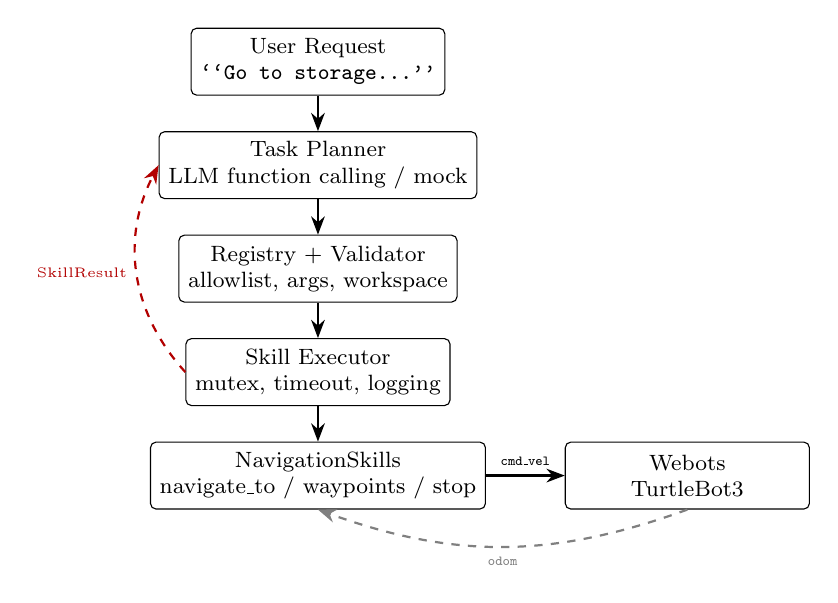
\begin{tikzpicture}[
  box/.style={draw, rounded corners=2pt, align=center, minimum width=3.1cm,
              minimum height=0.85cm, font=\footnotesize},
  arr/.style={-{Stealth}, thick},
  fb/.style={-{Stealth}, thick, dashed, red!70!black}
]
\node[box] (user) {User Request\\\texttt{``Go to storage...''}};
\node[box, below=0.45cm of user] (planner) {Task Planner\\LLM function calling / mock};
\node[box, below=0.45cm of planner] (valid) {Registry + Validator\\allowlist, args, workspace};
\node[box, below=0.45cm of valid] (exec) {Skill Executor\\mutex, timeout, logging};
\node[box, below=0.45cm of exec] (skills) {NavigationSkills\\navigate\_to / waypoints / stop};
\node[box, right=1.0cm of skills] (sim) {Webots\\TurtleBot3};
\draw[arr] (user) -- (planner);
\draw[arr] (planner) -- (valid);
\draw[arr] (valid) -- (exec);
\draw[arr] (exec) -- (skills);
\draw[arr] (skills) -- (sim) node[midway,above,font=\tiny]{\texttt{cmd\_vel}};
\draw[arr, dashed, gray] (sim.south) to[bend left=20]
      node[pos=0.5,below,font=\tiny]{\texttt{odom}} (skills.south);
\draw[fb] (exec.west) to[bend left=35]
      node[pos=0.5,left,font=\tiny]{SkillResult} (planner.west);
\end{tikzpicture}
\caption{System architecture: request $\rightarrow$ planner $\rightarrow$
validator/executor $\rightarrow$ skills $\rightarrow$ simulation, with
structured results fed back for recovery.}
\label{fig:arch}
\end{figure}

\subsection{Skill interface}
Each of the three skills (\texttt{navigate\_to(x, y, theta)},
\texttt{follow\_waypoints(waypoints)}, and \texttt{stop()}) is described by
a registry entry containing a description, typed parameters with
minimum/maximum bounds, preconditions, a success condition, and a timeout.
The workspace bounds are set from the physical walls of the Webots
TurtleBot3 house world (odom frame: west wall at $x=-1.36$, east wall at
$x=3.74$, south wall at $y=-5.1$, north wall at $y=5.1$). The validator uses
slightly extended limits ($x \in [-2,4]$, $y \in [-5.2,5.2]$) to provide a
safety margin, and rejects any target outside this measured area before it
reaches the robot. A call returns a \texttt{SkillResult} with a
\texttt{reason} enumeration (\texttt{ok}, \texttt{timeout},
\texttt{invalid\_arguments}, \texttt{precondition\_failed}, etc.) plus
measurable fields such as \texttt{position\_error\_m} and
\texttt{heading\_error\_rad}. The same registry generates three
machine-readable views (a compact registry for system prompts, OpenAI tool
schemas for function calling, and standard JSON Schema), keeping the three
views consistent with each other and with the validator.

% =====================================================================
% III. IMPLEMENTATION
% =====================================================================
\section{Implementation}

\subsection{Navigation (Part~2)}
\texttt{navigate\_to} reports success only when the position error and the
heading error are both within their tolerances ($0.1$\,m and $0.1$\,rad). In
the initial implementation the heading error was evaluated relative to the
instantaneous direction from the robot to the target. This caused false
successes: the robot could arrive at the target position facing the direction
of travel instead of the user-specified heading \texttt{theta}. To fix this,
the success condition now evaluates the heading error strictly against
\texttt{target\_theta}, and a separate in-place rotation phase is activated
after the robot reaches the target position to align it with
\texttt{target\_theta} before success is reported.

The controller is therefore a two-phase state machine with separate control
laws per axis: PD on the linear axis and a full PID on the angular axis.
While the robot is farther than the position tolerance from the target, it
first turns toward the target direction and then drives, with the speed scaled
down near the goal. The linear command is
$v=\mathrm{clamp}(0.35\,d+0.08\,\dot d,\,0.05,\,0.25)$\,m/s, a proportional
law on the remaining distance $d$ plus a derivative term on its rate of change
$\dot d$ that brakes early near the goal. The angular axis uses a discrete
PID ($K_p=1.0$, $K_i=0.02$, $K_d=0.03$) with an integral clamp of $0.5$, a
derivative limit of $1.5$\,rad/s, a dead-band of $0.02$\,rad, and a
$0.15$\,rad/s minimum-output floor so that small commands remain effective
despite wheel friction. While driving, small heading
errors are corrected continuously with a bounded steering term instead of
discrete stop-and-turn cycles, which removes the jerky motion observed when
correction was only applied above a hard threshold. Once inside the position
tolerance, the phase is locked into in-place rotation to the target heading,
with hysteresis ($0.25$\,m) so that small position drift does not make the
robot oscillate between driving and turning. This failure mode was observed in
an early version and caused timeouts. On timeout the robot stops and reports
the remaining position and heading errors.

\texttt{follow\_waypoints} visits each pose in order and reports
\texttt{last\_reached} and \texttt{failed\_at} indices on failure, dividing
its total timeout budget evenly among the waypoints. \texttt{stop()} publishes
a zero twist several times to guarantee the robot halts.

\subsection{Skill interface and executor (Part~3)}
Part~3 acts as a structured skill interface that decouples the high-level
task planner (Part~4) from the low-level control layer (Part~2). It provides
three functions: contract definition through a skill registry that specifies
names, typed parameters, preconditions, and timeouts; argument validation and
workspace-bound checking that reject malformed or out-of-range calls before
they reach the robot; and standardized result formatting that returns
structured JSON (success, reason, elapsed time) for every execution, enabling
the planner to make consistent recovery decisions. The interface layer is
implemented with Python dataclasses (typed, JSON-serializable, zero external
dependencies). The \texttt{SkillExecutor} is the only entry point to the
robot: it checks the allowlist, validates arguments (types, ranges,
workspace, and the structure of waypoints), enforces mutual exclusion (a
second skill call while busy is rejected with \texttt{precondition\_failed},
except \texttt{stop}), applies an enforced timeout, and appends one JSON line
per call (\texttt{logs/skill\_calls.jsonl}).

\subsection{LLM tool calling and safety (Part~4)}
The planner calls an OpenAI-compatible API (DeepSeek \texttt{deepseek-chat})
with \texttt{tools=tool\_schemas()}. The LLM only proposes calls. The loop
executes each call through the executor and feeds the \texttt{SkillResult}
back, repeating until the model replies with a final message. At most
\texttt{max\_steps} tool calls are allowed per task, and at most one retry per
failing skill, so a misbehaving model cannot keep the robot busy indefinitely.
The mock planner used during development emits the same call
format, so the validator, executor, and recovery paths are exercised
identically in offline tests without an API key. Recovery is rule-based and
bounded: \texttt{timeout} $\rightarrow$ retry once $\rightarrow$ if it fails
again, stop and report; \texttt{invalid\_arguments} or unknown skills
$\rightarrow$ reject the step and abort the plan. An early failure in which
the model produced waypoints with missing headings was fixed by making each
waypoint an object $\{x, y, theta\}$ in the tool schema, which the validator
also enforces. Dispatch is restricted to the three registered methods. The
executor never evaluates or executes code generated by the model. Every task
run additionally records the original plan, per-step results, recovery
decision, and final outcome in \texttt{logs/task\_planner.jsonl}.

\subsection{Validation and rejection classes}
Calls are rejected with a typed reason before any command is published:
\texttt{unknown\_skill} for a call outside the fixed allowlist (for example
\texttt{teleport}), \texttt{invalid\_arguments} for wrong types, missing
parameters, targets outside the measured workspace, or waypoints that are not
\texttt{\{x, y, theta\}} objects, and \texttt{precondition\_failed} when a
second call arrives while the robot is busy. These classes map one-to-one to
the required safety checks (allowlist, typed arguments, workspace bounds, and
bounded step and retry counts). Each rejection leaves the robot stationary.
One live case, waypoints generated without \texttt{theta}, is discussed in
Section IV.

% =====================================================================
% IV. EXPERIMENTS AND RESULTS
% =====================================================================
\section{Experiments and Results}

\subsection{Setup}
Experiments ran in an Ubuntu 22.04 virtual machine with ROS~2 Humble and the
Webots \emph{TurtleBot3 Burger} house world. Basic motion was first verified
by keyboard teleoperation in the same environment (Part~1). The robot spawns
at the origin of the odometry frame. Four named locations
(\texttt{entrance}, \texttt{storage}, \texttt{workbench},
\texttt{charging\_station}) were placed in obstacle-free areas verified by a
clearance checker over all pairwise straight-line paths
($\ge 0.35$\,m from all walls and furniture). Because navigation follows
straight lines without obstacle avoidance, this manual placement guarantees
that every commanded path is collision-free by construction. The LLM used is
DeepSeek \texttt{deepseek-chat} \cite{deepseek} through the OpenAI-compatible
API \cite{openai-fc}.

\subsection{Test cases}
Table~\ref{tab:nav} reports the navigation accuracy of the Part~2 skills in the
Webots simulator: reaching a target is reported only when the position error is
$\le 0.1$\,m \emph{and} the heading error is $\le 0.1$\,rad, including the
heading-alignment case ($\theta = \pi/2$) that exercises the in-place
rotation phase.

\begin{table}[t]
\centering
\caption{Navigation accuracy in the Webots simulator (Part~2).}
\label{tab:nav}
\footnotesize
\resizebox{\columnwidth}{!}{%
\begin{tabular}{@{}lccc@{}}
\toprule
Target (pose) & Elapsed (s) & pos err (m) & hdg err (rad) \\
\midrule
entrance ($-0.7, -1.6, \pi$) & 17.4 & 0.086 & 0.099 \\
storage ($0.0, -3.2, 0$) & 17.5 & 0.087 & 0.090 \\
workbench ($1.5, -2.8, \pi/2$) & 14.9 & 0.086 & 0.086 \\
charging\_station ($2.2, -3.5, 0$) & 13.8 & 0.084 & 0.096 \\
\bottomrule
\end{tabular}}
\par\vspace{2pt}
\footnotesize Note: each named location was reached within the
\texttt{navigate\_to} tolerances ($0.1$\,m, $0.1$\,rad) in the Webots
simulator. Measured errors across these runs were $0.084$--$0.087$\,m
(position) and $0.086$--$0.099$\,rad (heading). Additional task-level runs
(see Table~\ref{tab:results}) measured position errors up to $0.099$\,m and
heading errors within the same $0.086$--$0.099$\,rad band.
\end{table}

Table~\ref{tab:results} evaluates the main links in the execution pipeline
rather than only the end-to-end success rate. The single-location request
exercises natural-language grounding and basic skill selection, the
multi-location request exercises sequential task planning and execution, the
unknown-location case exercises pre-execution validation, and the timeout
scenario exercises bounded recovery. The malformed-waypoint case (Section
IV) further tests whether schema-level errors are intercepted before
reaching the robot. Together these cases cover planning, execution,
validation, and recovery within the implemented system.

\begin{table}[t]
\centering
\caption{Results in the Webots simulator.}
\label{tab:results}
\footnotesize
\resizebox{\columnwidth}{!}{%
\begin{tabular}{@{}lccc@{}}
\toprule
Request (mode) & Outcome & Time (s) & Recovery \\
\midrule
Go to storage (mock) & success & 24.5 & --- \\
Workbench, storage, stop (mock) & success & 31.3 & --- \\
Go to kitchen (mock) & rejected & 0.0 & reject \\
Go to storage (LLM) & success & 26.5 & retry once \\
Workbench, storage, stop (LLM) & success & 34.4 & --- \\
Go to kitchen (LLM) & rejected & 0.5 & reject \\
timeout scenario (offline) & failed & 0.8 & retry, stop+report \\
\bottomrule
\end{tabular}}
\par\vspace{2pt}
\footnotesize Note: in the LLM run of \texttt{Go to storage.}, the first
navigation attempt timed out (20.2\,s) and the planner retried once, which
succeeded; the retry is therefore listed as a recovery action although the
task outcome is success.
\end{table}

\subsection{Analysis}
All three required requests succeed in both modes. The robot reaches every
target with position error $\le 0.1$\,m and heading error $\le 0.1$\,rad
(e.g., \texttt{position\_error\_m} $=0.087$,
\texttt{heading\_error\_rad} $=0.099$ for the workbench in the LLM run), which
validates the heading-alignment fix. The invalid location ``kitchen'' is
rejected without moving the robot: the mock planner lists valid
locations, and the LLM independently refuses with
``invalid location: kitchen''. The bounded recovery path was exercised:
after a navigation timeout the planner retried once, and when the retry also
failed it stopped and reported. A second failure case, the LLM emitting
waypoints with missing headings, was intercepted by the validator
(\texttt{invalid\_arguments} $\rightarrow$ \texttt{reject\_step}), and fixing
the tool schema to object-form waypoints made the same request succeed.
This case shows that the validator catches such failures before any command
is sent. Repeated runs of the same instruction were consistent: the mock
planner's \texttt{Go to storage.} completed in 24.5 and 24.7\,s in two
sessions and in 26.5\,s with the LLM. The small difference is expected: the
LLM path adds API round-trip latency, and for the multi-location request the
LLM may choose a different (but equivalent) skill sequence such as a single
\texttt{follow\_waypoints} call instead of two \texttt{navigate\_to} calls,
so wall-clock time is not directly comparable between modes. Every run
converged within the stated tolerances, with measured position errors in
$0.084$--$0.099$\,m and heading errors in $0.086$--$0.099$\,rad.
For every task the planner log records the original plan, per-step results,
recovery decision, and final outcome, which supports auditing and
reproduction. Taken together, these results suggest that the
validator--executor boundary decouples LLM output variability
from low-level robot safety, while retaining enough flexibility for the
required natural-language tasks: the model can plan freely, but every action
that reaches the robot is deterministic, validated, and logged.

The mock-versus-LLM comparison also illustrates the underlying engineering
trade-off. The mock planner is deterministic and fast, but limited to
predefined task patterns; the LLM planner adds latency and nondeterminism
in exchange for natural-language flexibility and variable skill sequences.
The role of the validator--executor boundary is therefore not to remove
this variability but to contain it at the planning layer, keeping robot
execution constrained, observable, and recoverable.

% =====================================================================
% V. LIMITATIONS AND FUTURE WORK
% =====================================================================
\section{Conclusion and Future Work}
We built and validated a safe, modular LLM-assisted robot task planning
system in simulation. Every proposed skill call passes an executor gate
(allowlist, argument validation, preconditions, guarded execution, structured
results with logging) before the robot moves. In Webots experiments all
required requests succeeded within $0.1$\,m position and $0.1$\,rad heading
error, and invalid or out-of-range requests were rejected without robot
motion. The main contribution is a reproducible engineering architecture
that combines function-calling LLMs with explicit skill contracts and
bounded recovery, yielding a system that is safe in practice and
reproducible.

Recalling the four design goals from Section~I, the system achieves
safety by confining the LLM to a fixed allowlist and validating every
call before execution; explicit contracts through the registry's
typed parameters, preconditions, and structured results; reliable
navigation by reporting success only within the position and heading
tolerances and handling timeouts safely; and modularity by decoupling
the control, interface, and planning layers so that each part can be tested
independently. The evaluation provides evidence that these goals are
supported in the implemented system: the required requests succeed within
tolerance, and invalid or out-of-range requests never move the robot.

The current system has no obstacle avoidance: navigation follows straight
lines, so locations must be manually selected in obstacle-free areas. A
lidar-based local avoidance or a navigation stack would remove this
constraint. Locations are hard-coded instead of discovered from a map, and
the planner is single-request and stateless. LLM behavior is nondeterministic,
so the validator must remain strict. Recovery is rule-based and does not yet
let the model repair its own plan. A further direction is state-aware
validation: the current validator checks syntax, ranges, the allowlist, and
the workspace, but a legally typed argument is not necessarily feasible in
the robot's current state; checking the robot's pose and path feasibility
against an obstacle map before execution would tighten the safety boundary
once such a map becomes available. Future work also includes
occupancy-map based planning, multi-request stateful dialogues, learned
recovery policies, and migration to a physical robot, since the executor
already accepts any robot driver that provides the three skill methods. As a
safety consideration, API credentials are supplied through environment
variables only and are never stored in the repository.

% =====================================================================
% REFERENCES
% =====================================================================
\begin{thebibliography}{6}
\bibitem{saycan} M. Ahn et al., ``Do as I Can, Not as I Say: Grounding
Language in Robotic Affordances,'' arXiv:2204.01691, 2022. [Online].
Available: \url{https://arxiv.org/abs/2204.01691}
\bibitem{rt2} A. Brohan et al., ``RT-2: Vision-Language-Action Models Transfer
Web Knowledge to Robotic Control,'' arXiv:2307.15818, 2023. [Online].
Available: \url{https://arxiv.org/abs/2307.15818}
\bibitem{voyager} G. Wang et al., ``Voyager: An Open-Ended Embodied Agent with
Large Language Models,'' arXiv:2305.16291, 2023. [Online]. Available:
\url{https://arxiv.org/abs/2305.16291}
\bibitem{cap} J. Liang et al., ``Code as Policies: Language Model Programs for
Embodied Control,'' arXiv:2209.07753, 2022. [Online]. Available:
\url{https://arxiv.org/abs/2209.07753}
\bibitem{deepseek} DeepSeek, ``API Documentation.'' [Online]. Available:
\url{https://api-docs.deepseek.com/} (Accessed: Sep.\ 2026)
\bibitem{openai-fc} OpenAI, ``Function calling.'' [Online]. Available:
\url{https://platform.openai.com/docs/guides/function-calling}
(Accessed: Sep.\ 2026)
\end{thebibliography}

\end{document}
